\documentclass[UTF8]{ctexart}
\usepackage{subfigure}
\usepackage{caption}
\usepackage{amsmath,bm}
\usepackage{amssymb}
\usepackage{pifont}
\usepackage{geometry}
\usepackage{graphicx}
\usepackage{gensymb}
\usepackage{wrapfig}
\usepackage{titlesec}
\usepackage{float}
\usepackage{diagbox}
\usepackage{fancyhdr}
\usepackage{color}
\usepackage{bm}
\pagestyle{plain}
\geometry{a4paper,scale=0.8}
\CTEXsetup[format+={\raggedright}]{section} 
\title{通网2021期中}
\author{Deschain}
\titlespacing*{\section}
{0pt}{0pt}{0pt}
\titlespacing*{\subsection}
{0pt}{0pt}{0pt}
\titlespacing*{\paragraph}
{0pt}{0pt}{0pt}
\titlespacing*{\subparagraph}
{0pt}{0pt}{0pt}
\titleformat*{\section}{\normalsize}
\begin{document}
\maketitle
\section*{}
1.有一数字线性基带传输系统,采用升余弦脉冲成形滤波器,滚降系数为$\alpha$,带宽约束为$W$,符号
集合的大小为$M$,试计算:\\
(1)当$\alpha=0.2,M=8,W=3MHz$是,采样点无失真传输条件下的符号率最高为多少?\\
(2)当$\alpha=1,M=16$时,单位带宽承载的bit速率为多少?\\
(3)当$W=24kHz,M=4$时,在保证接收采样点无失真的情况下,传输1路标准PCM(传输速率64kbps)所能允
许的最大滚降系数$\alpha$为多少?\\
2.已知某非对称二元信道(Binary Non-Symmetric Channel),信道条件概率矩阵$P(Y\lvert X)$
\begin{equation*}
  \begin{aligned}
     & \begin{bmatrix}
      P(0\lvert0) & P(1\lvert0) \\
      P(0\lvert1) & P(1\lvert1) \\
    \end{bmatrix}=
    \begin{bmatrix}
      0.3 & 0.7 \\
      0.4 & 0.6 \\
    \end{bmatrix}
  \end{aligned}
\end{equation*}
输入符号$X$的概率分布服从
\begin{equation*}
  \begin{aligned}
     & \begin{pmatrix}
      x_1 & x_2 \\
      P_1 & P_2 \\
    \end{pmatrix}=
    \begin{pmatrix}
      0   & 1   \\
      0.2 & 0.8 \\
    \end{pmatrix}
  \end{aligned}
\end{equation*}
求:\\
(1)输出符号集$Y$的平均信息量$H(Y)$;\\
(2)条件熵$H(X\lvert Y),H(Y\lvert X)$,以及$X$和$Y$的联合熵$H(XY)$;\\
(3)输入符号$X$和输出符号$Y$的平均互信息量$I(X;Y)$。\\
3.对概率密度函数如图1所示的随机变量$x$进行量化。若采用两电平量化,且分层电平为0,试求最优(量化
均方噪声最小)的重建电平$x_1$和$x_2$。\\
\begin{figure}[H]
  \centering
  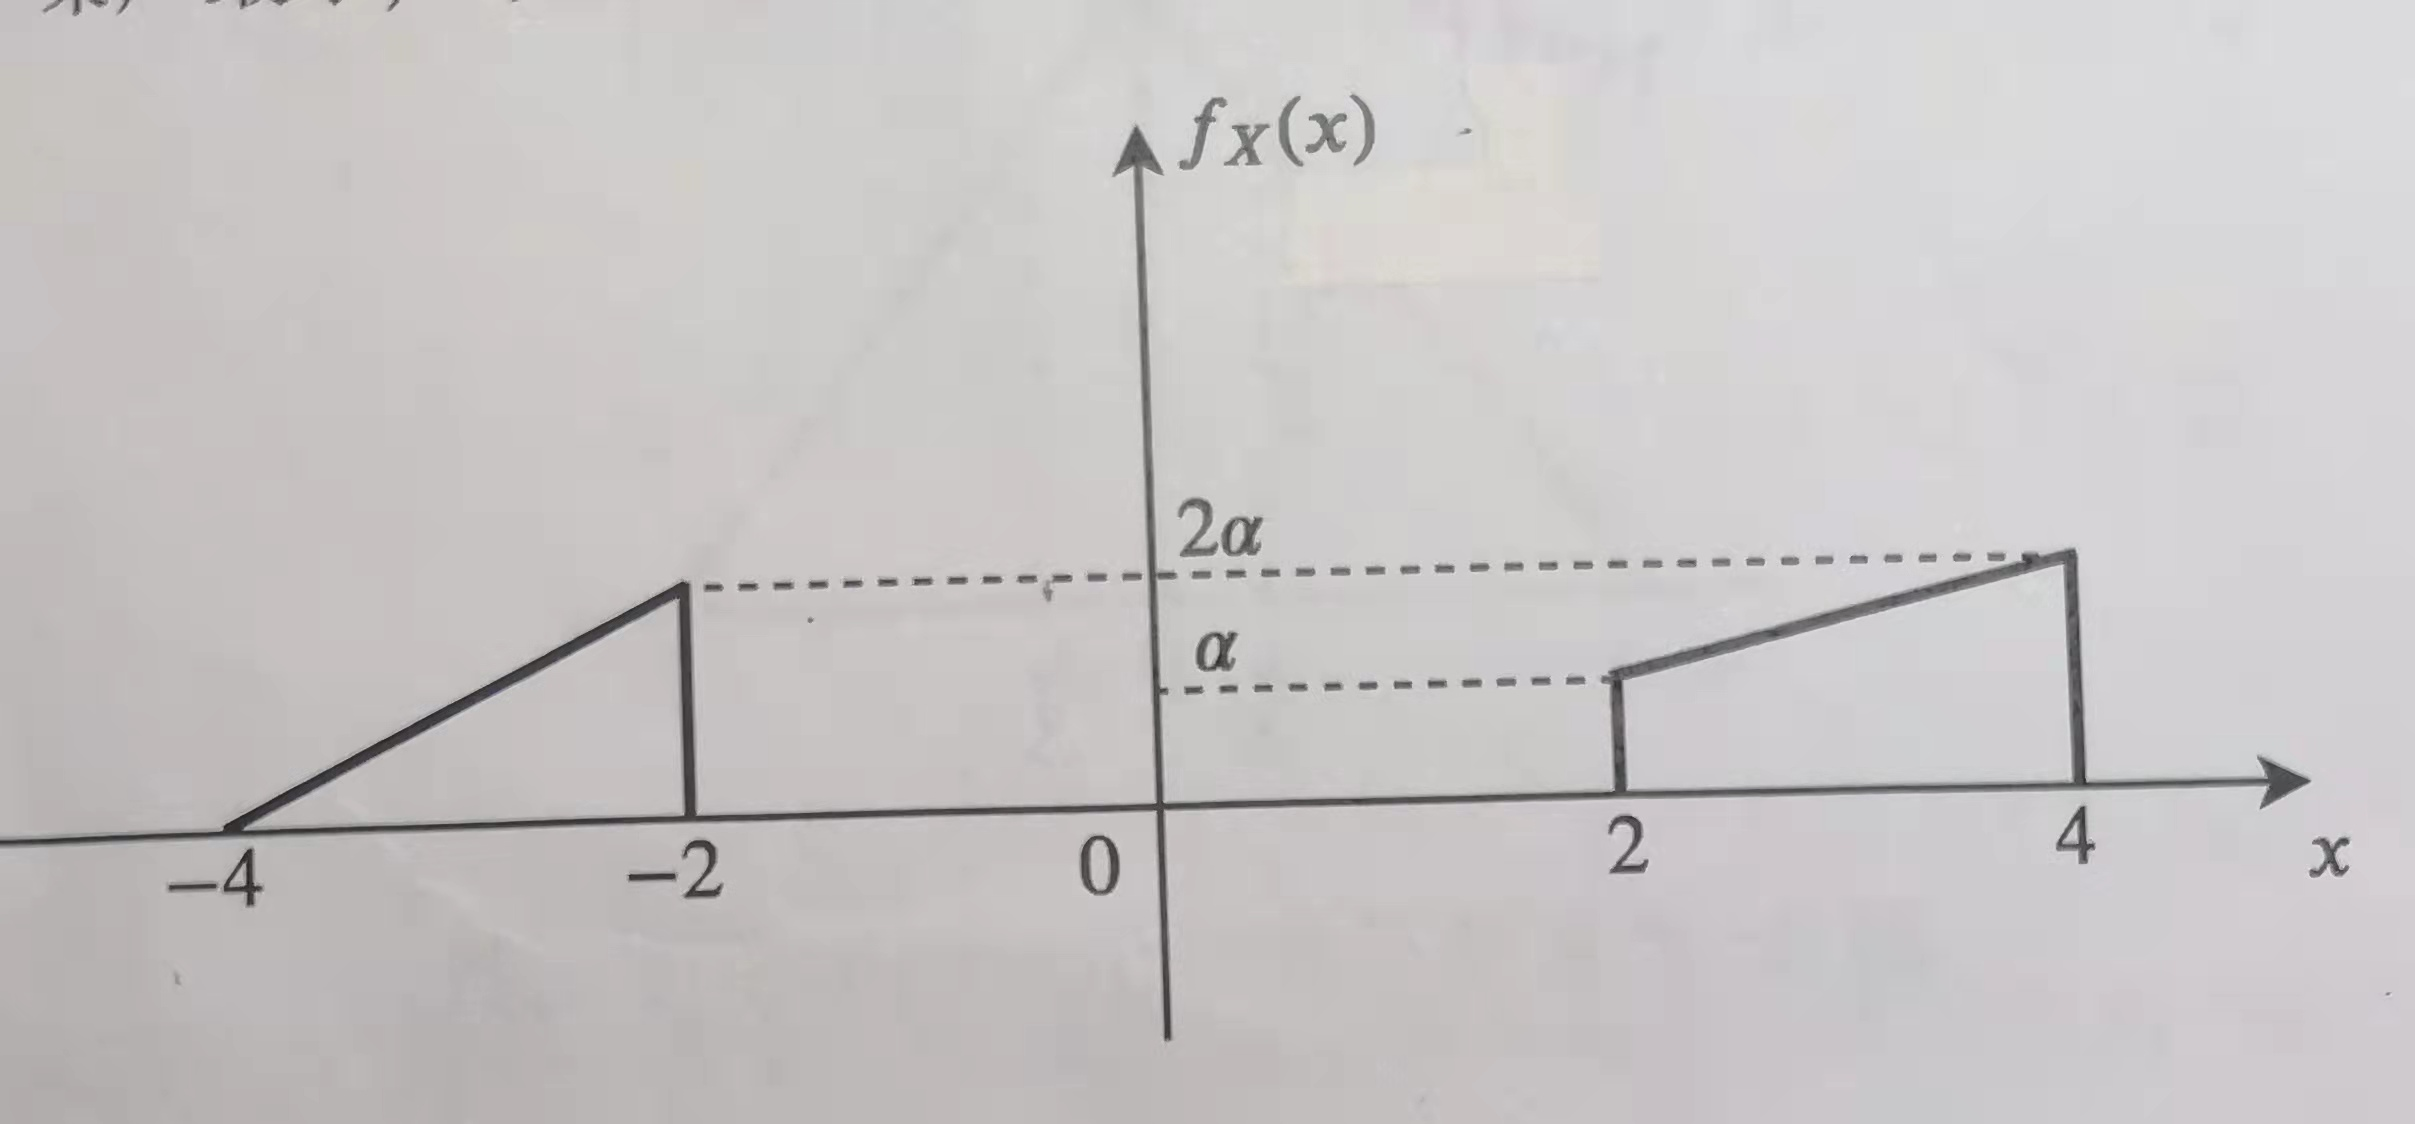
\includegraphics[width=10cm,height=4cm]{1.jpg}
  \caption*{图1:概率密度函数}
\end{figure}
\section*{}
4.考虑图2所示的星座图,已知每个星座点(复电平点)等概出现。\\
(1)已知(a)、(b)两星座图中的$\alpha$相同,请比较(a)、(b)两星座图在通过相同的加性复高斯噪声信道
(噪声时序部独立同分布)最佳判决的误符号率大小,并证明你的结论。\\
(2)试求(a)、(b)两星座图下基带平均发送功率比(除星座图设计不同外,基带脉冲能量、符号速率等其余
相关条件均相同)。\\
\begin{figure}[H]
  \centering
  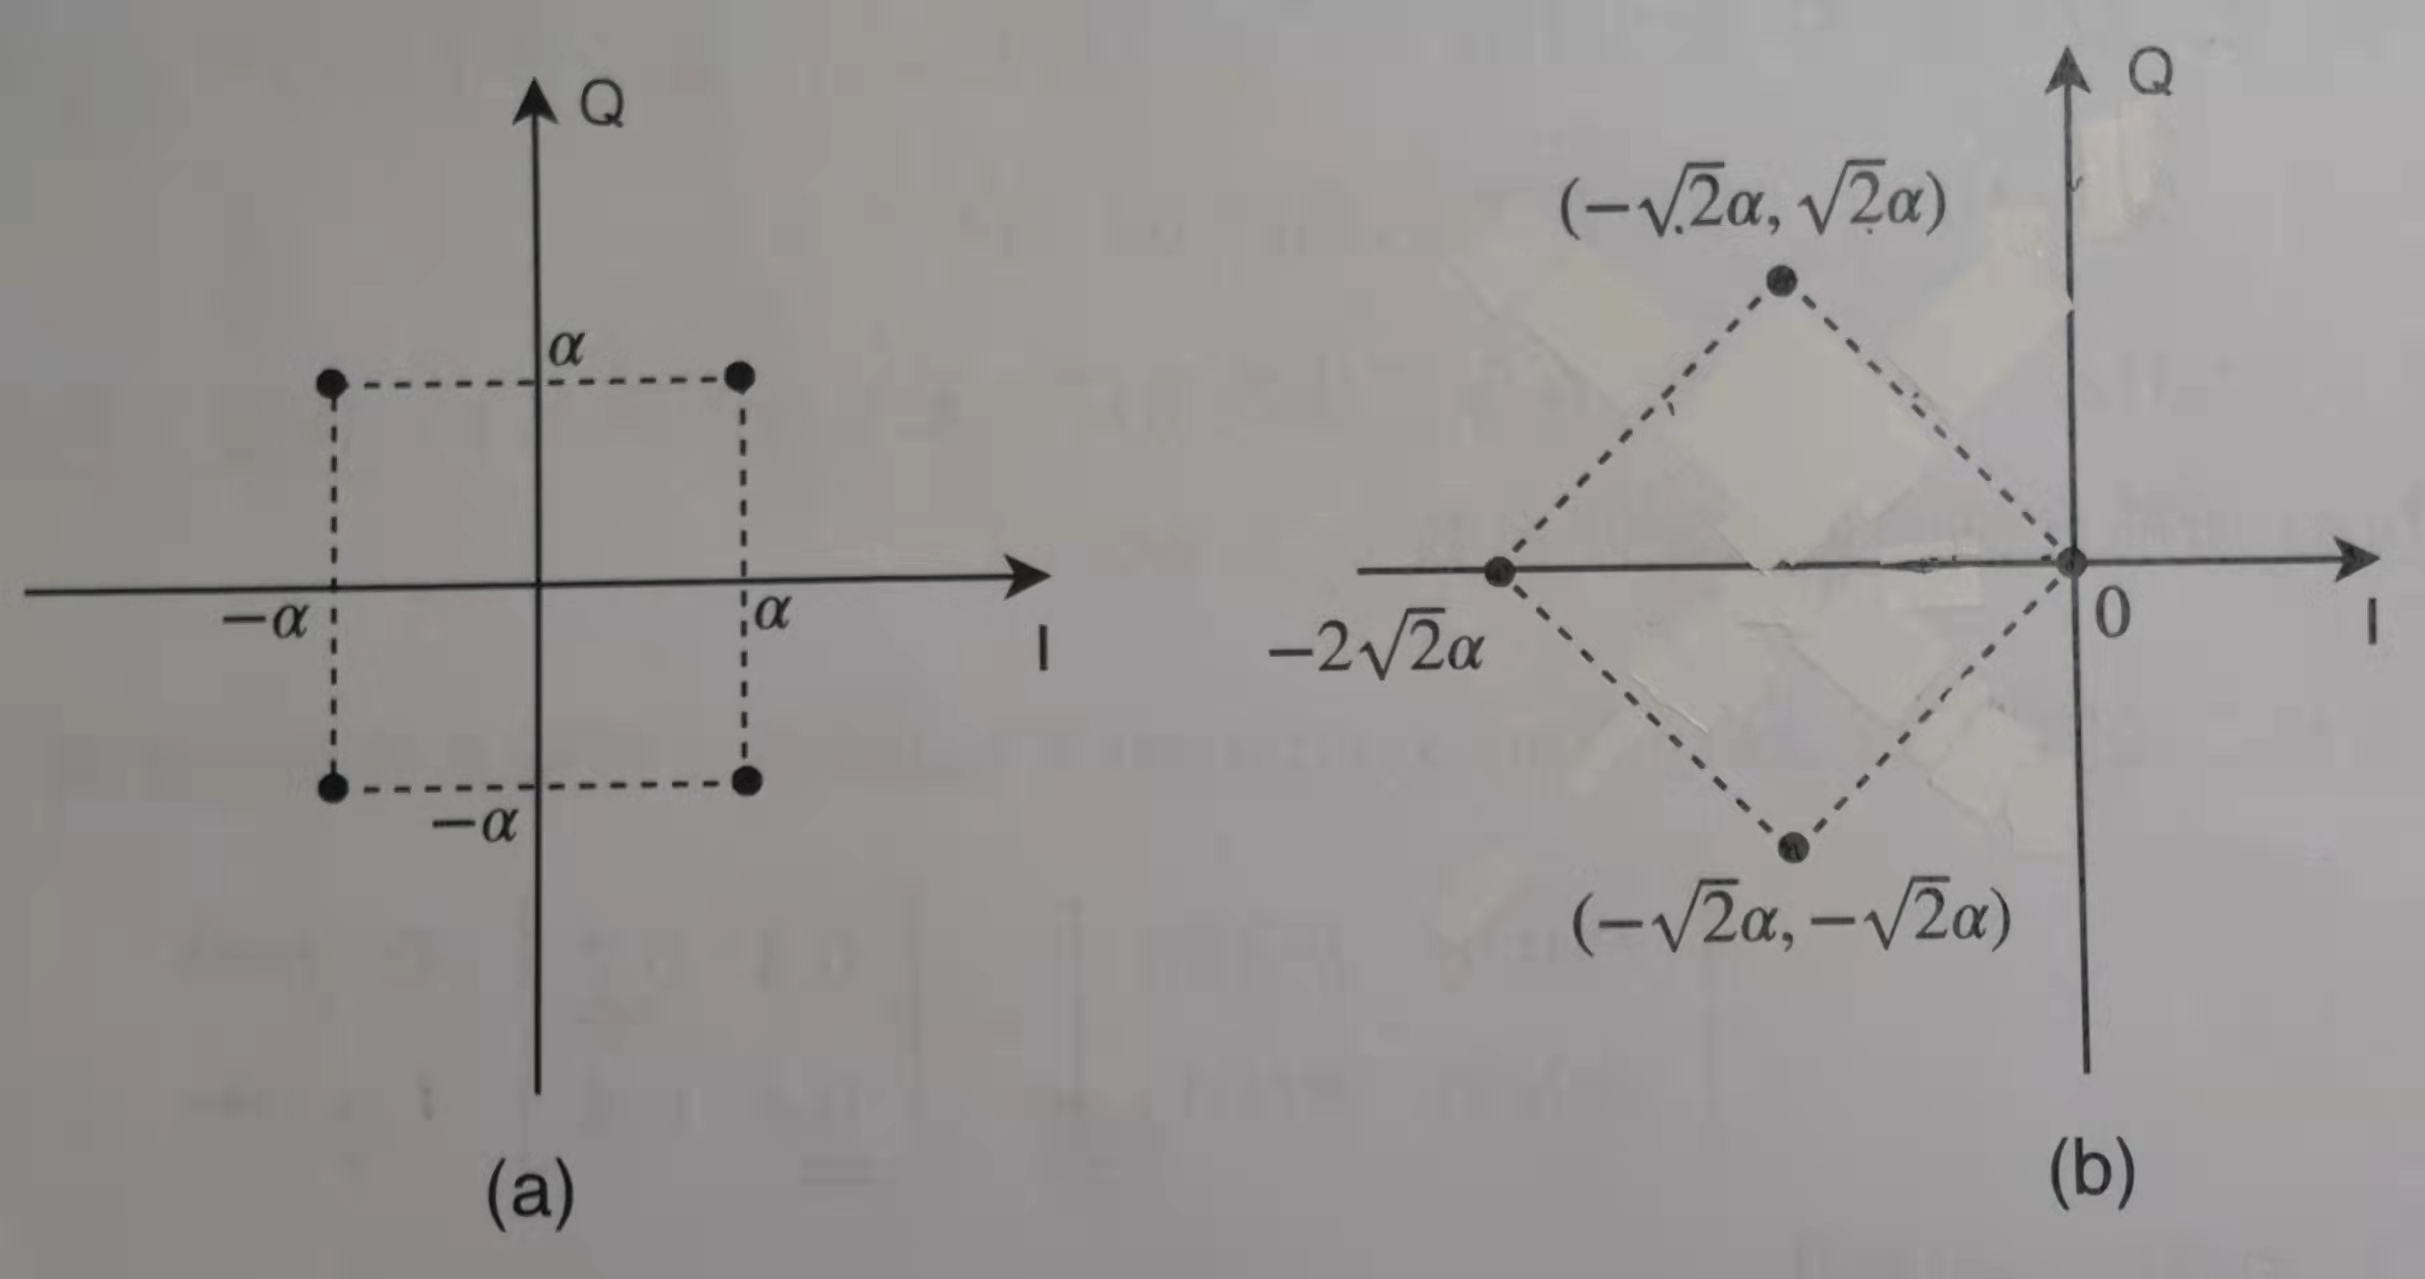
\includegraphics[width=12cm,height=6cm]{2.jpg}
  \caption*{图2:星座图}
\end{figure}
\section*{}
5.已知模拟信号抽样值的概率密度函数如题图3所示。采用三电平量化器对抽样值进行量化,量化区间为$I_1
  =(-1,-\frac{1}{3}],I_2=(-\frac{1}{3},\frac{1}{3}]$以及$I_1=(\frac{1}{3},1]$。在此量化区间
设计的基础上。\\
(1)请设计重建电平使得输入信号与量化噪声功率比为SNR最大,并给出量化噪声功率和信噪比SNR;\\
(2)求量化器输出符号的熵。\\
\begin{figure}[H]
  \centering
  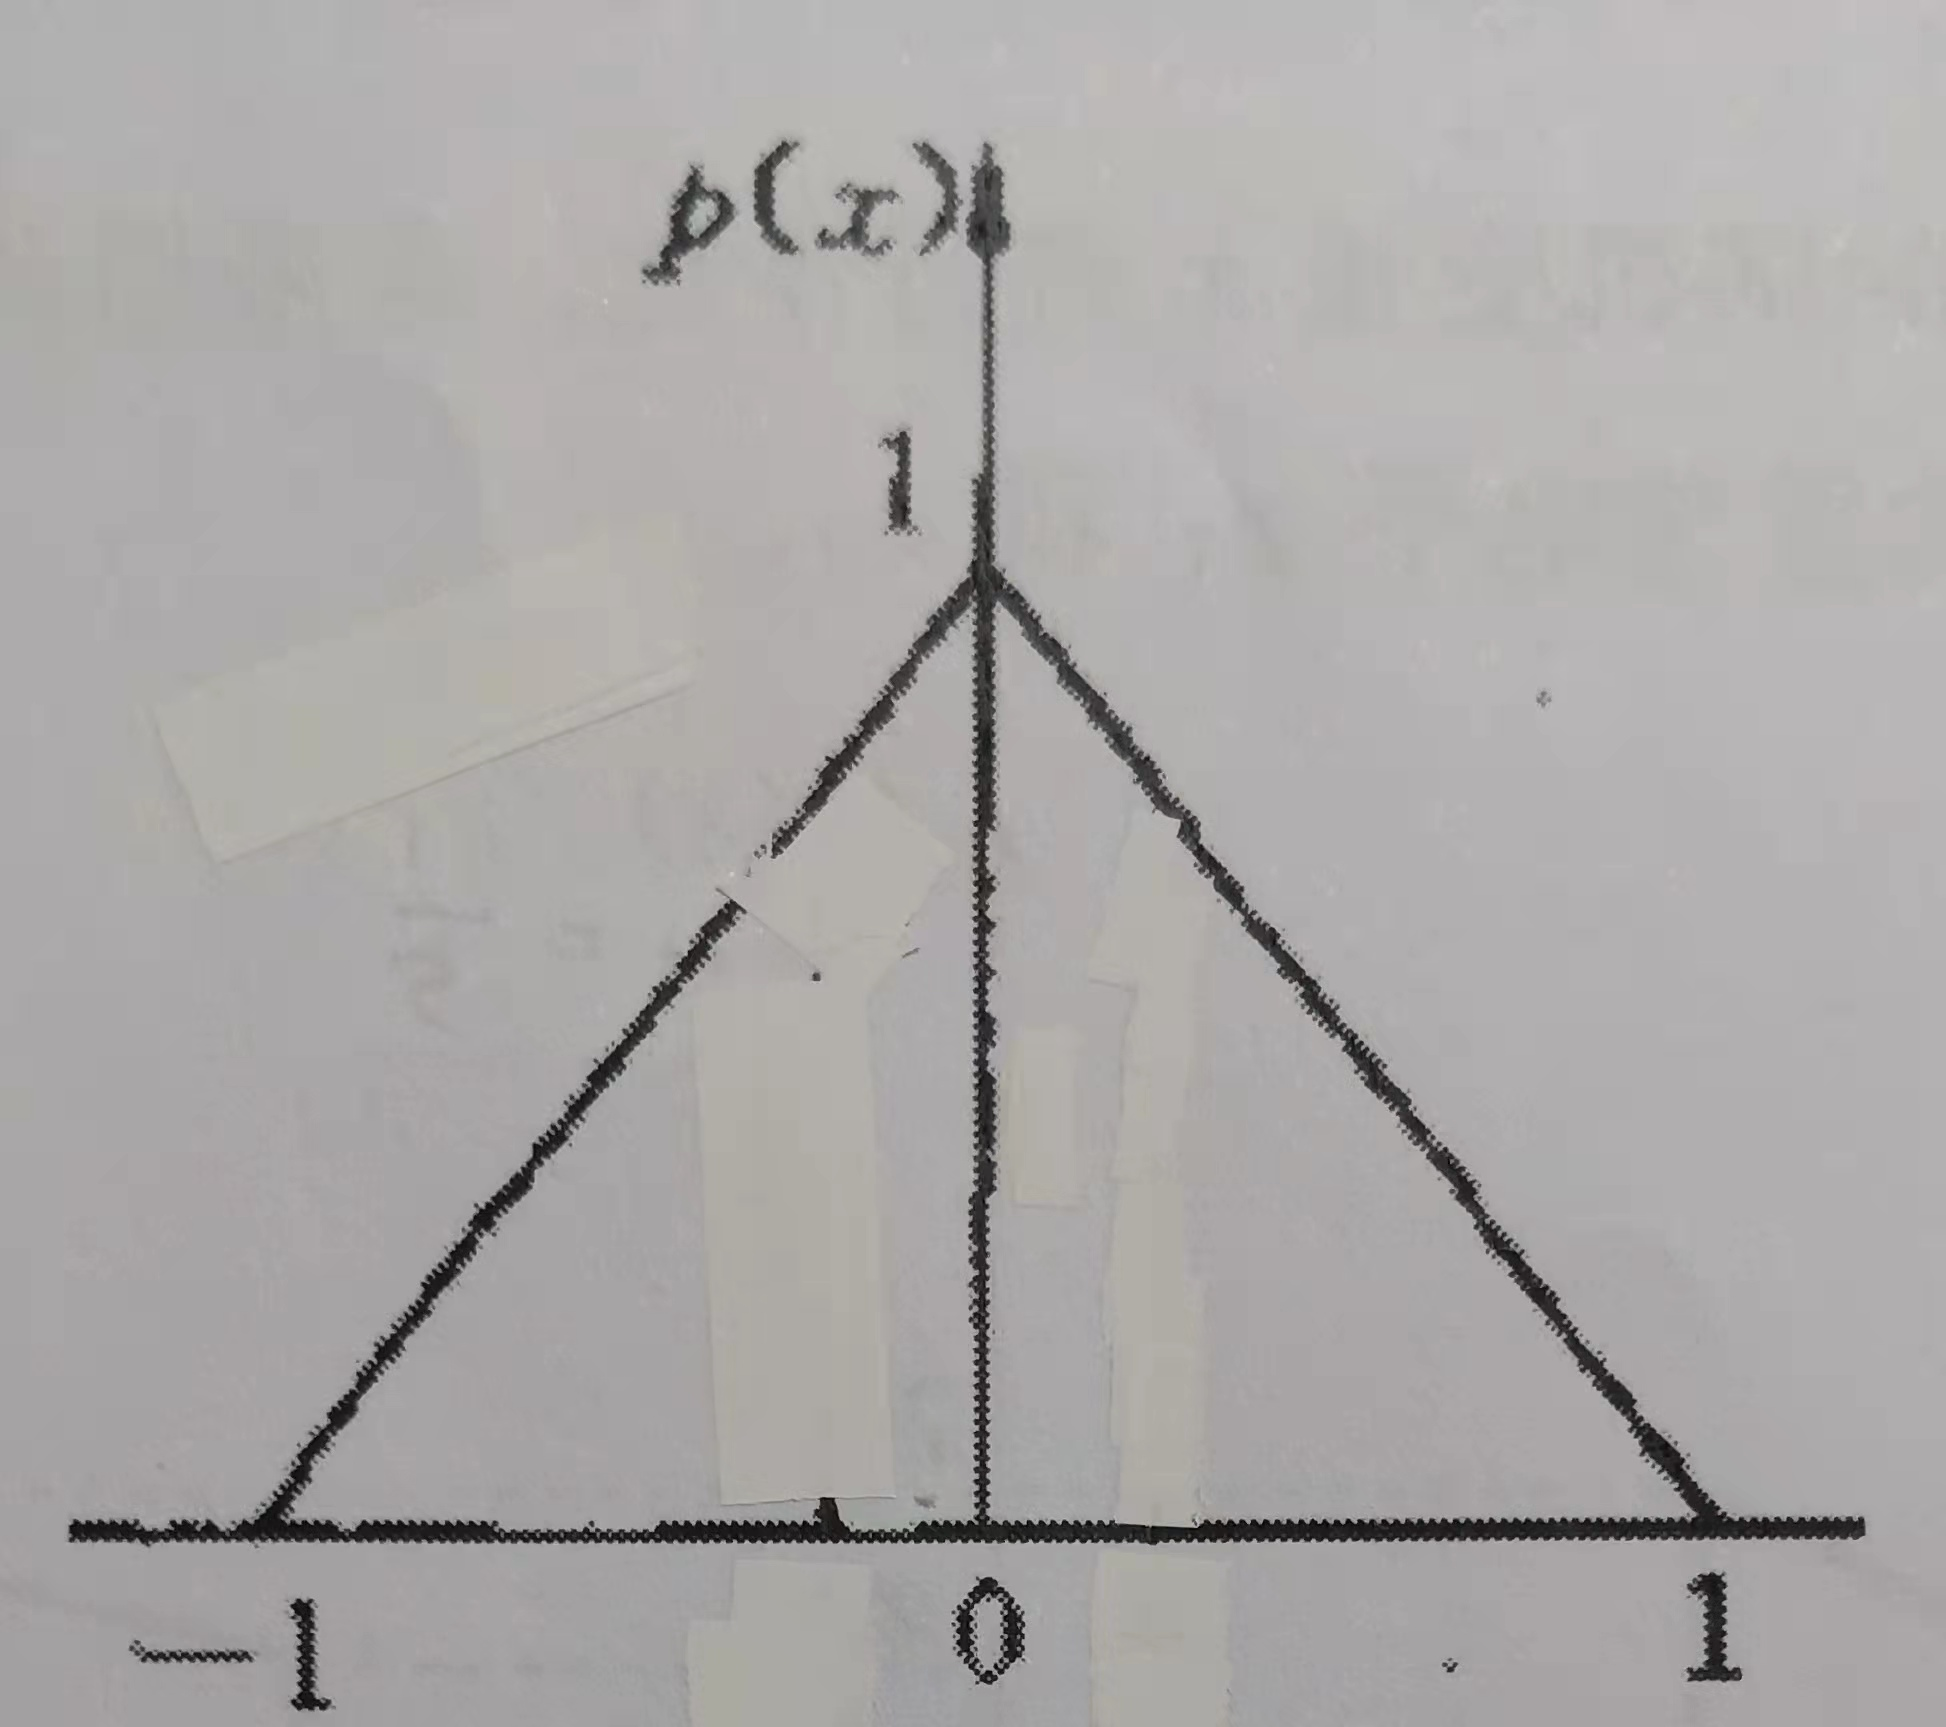
\includegraphics[width=6cm,height=5cm]{3.jpg}
  \caption*{图3:模拟信号抽样值的概率密度函数}
\end{figure}
\section*{}
6.考虑一个由$N$个独立的子信道组成的串行系统,输入和输出分别为$X,Y$。\\
(1)若$X,Y$取值范围为$\{0,1\}$,每个子信道为错误概率为$p$的二元对称信道,如图4,。求串行信道的
信道容量$C_N$以及$\lim_{N\to\infty}(C_N)^{\frac{1}{N}}$。\\
\begin{figure}[H]
  \centering
  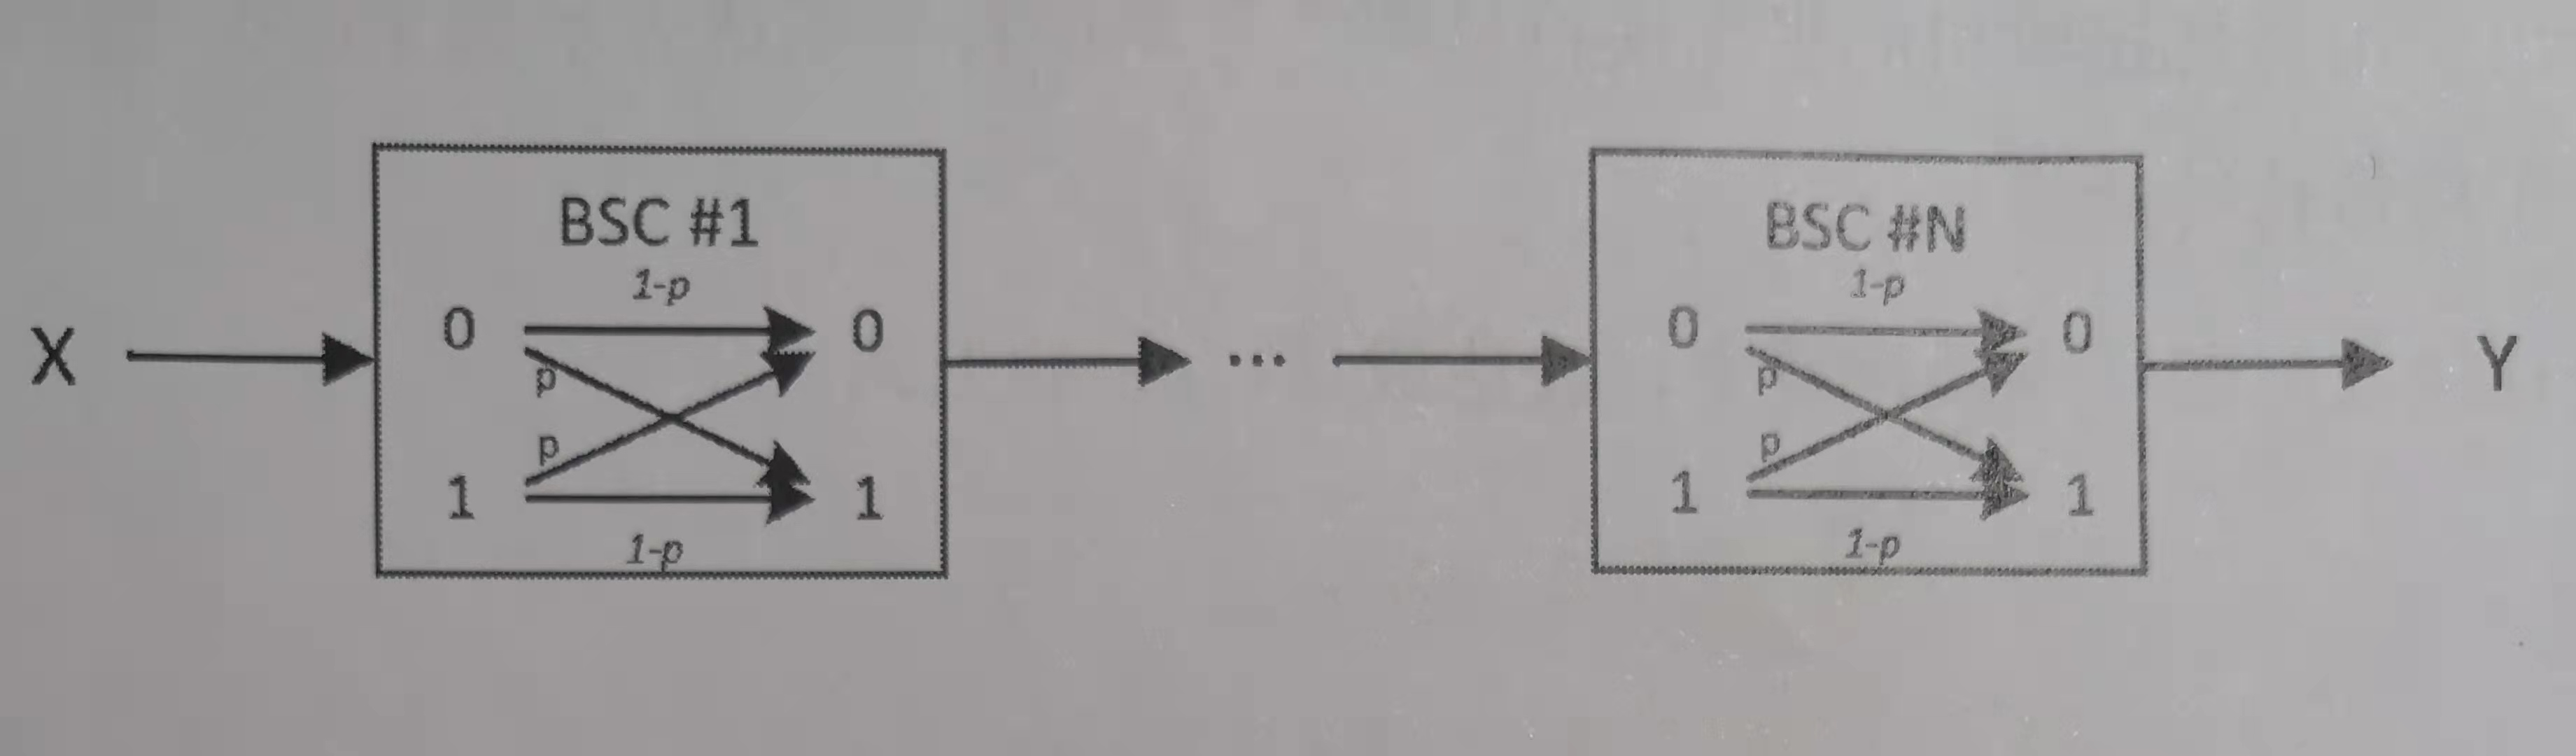
\includegraphics[width=12cm,height=3cm]{4.jpg}
  \caption*{图4:二元对称级联信道}
\end{figure}
(2)若$X,Y$取值范围为$\mathbb{R}$且$E(X^2)=P$,每个子信道为加性高斯噪声信道,噪声方差为$
  \sigma^2$,如图5。求串行信道的信道容量$C_N$以及$\lim_{N\to\infty}NC_N$。\\
\begin{figure}[H]
  \centering
  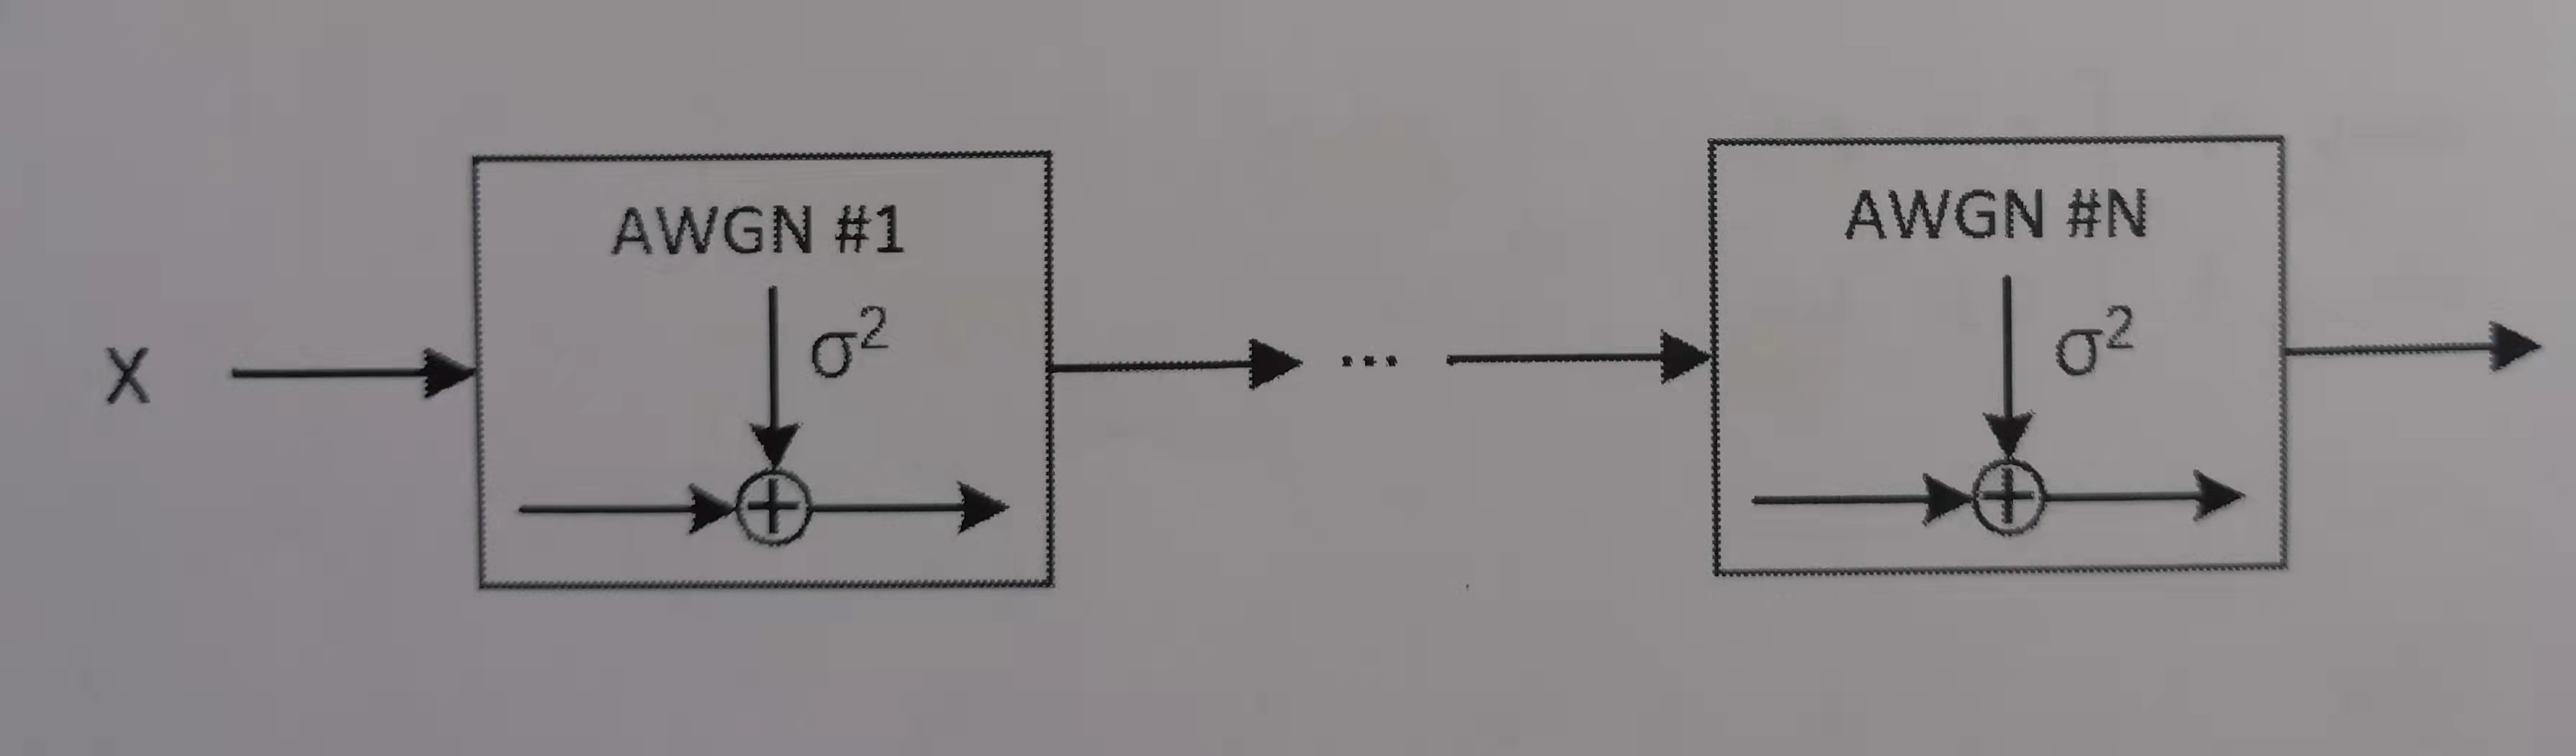
\includegraphics[width=12cm,height=3cm]{5.jpg}
  \caption*{图5:AWGN级联信道}
\end{figure}
7.某基带传输系统中,信源独立等概输出比特“0”与“1”。在该基带传输系统中。考虑使用四元基带调制,将
每个码元间隔$T_s$内的两个信息比特映射为波形$s_1(t),s_2(t),s_3(t),s_4(t)$之一。波形函数如下:
\begin{equation*}
  \begin{aligned}
     & s_1(t)=2\sqrt3A(\frac{Kt}{T_s}-\lfloor\frac{Kt}{T_s}\rfloor-\frac{1}{2})+A,
    0\leq t\leq T_s                                                                 \\
     & s_2(t)=-2\sqrt3A(\frac{Kt}{T_s}-\lfloor\frac{Kt}{T_s}\rfloor-\frac{1}{2})+A,
    0\leq t\leq T_s                                                                 \\
     & s_1(t)=-2\sqrt3A(\frac{Kt}{T_s}-\lfloor\frac{Kt}{T_s}\rfloor-\frac{1}{2})-A,
    0\leq t\leq T_s                                                                 \\
     & s_1(t)=2\sqrt3A(\frac{Kt}{T_s}-\lfloor\frac{Kt}{T_s}\rfloor-\frac{1}{2})-A,
    0\leq t\leq T_s                                                                 \\
  \end{aligned}
\end{equation*}
其中,$A$为某正常数,$K$为某正整数。在该四元基带调制中,比特序列“00”映射为$s_1(t)$,“01”映射
为$s_2(t)$,“11”映射为$s_3(t)$,“10”映射为$s_4(t)$。传输信道为单边噪声功率谱为$n_0$的加性高
斯白噪声信道。请完成如下题目:\\
(1)请画出$K=2$时,一个码元周期内的$s_1(t),s_2(t),s_3(t)$和$s_4(t)$的波形;\\
(2)根据调制波性特点,请设计出最优接收机结构与相应判决准则,以最小化误符号率;\\
(3)请给出使用最优接收机的平均误符号率(平均误符号率请表示为$\frac{E_b}{n_0}$的函数,其中,$E_b
$表示平均每比特能量)。\\
(4)求最佳接收时的平均误比特率,表达成$\frac{E_b}{n_0}$的形式。\\
\end{document}